% Results section for the NeurIPS draft.
% Primary claim: RePaint resampling interacts with conditioning type.

\section{Experiments}
\label{sec:experiments}

\subsection{Setup}
\label{sec:setup}
Models, training, and the full $(j,r,\mathrm{cr})$ grid are as in Section~\ref{sec:method}.
Unless noted, the headline comparisons use full reverse length $T{=}1000$, $j{=}10$, and center masks with $\mathrm{cr}\in\{0.40,0.50\}$.
We report image-wide PSNR and LPIPS~\citep{zhang2018lpips} (AlexNet; lower is better).

\paragraph{Paired comparisons.}
Every $\Delta$ in Table~\ref{tab:resampling-delta} is computed on the \emph{same} $n{=}32$ images, masks, and seeds under two resampling settings.
Per-sample seeding is held fixed across runs so that the only intentional change is the RePaint resampling count $r$.

\paragraph{Choice of comparison points.}
The $\Delta$ endpoints are \textbf{not} uniform across model types.
We compare each model at its practically relevant operating points suggested by the $r$-sweep in Figure~\ref{fig:lpips-heatmap}:
\begin{itemize}
  \item \textbf{Conditioned:} $\Delta = \mathrm{metric}(r{=}10) - \mathrm{metric}(r{=}1)$.
  \item \textbf{Unconditional:} $\Delta = \mathrm{metric}(r{=}5) - \mathrm{metric}(r{=}1)$.
\end{itemize}
Thus positive $\Delta$PSNR (resp.\ negative $\Delta$LPIPS) means the higher-$r$ setting improves over $r{=}1$ for that model.

\subsection{Resampling interacts with conditioning}
\label{sec:resampling-interaction}
Table~\ref{tab:resampling-delta} summarizes the paired effect of increasing $r$.
On conditioned models, moving from $r{=}1$ to $r{=}10$ \emph{degrades} quality: $\Delta\mathrm{PSNR}{=}{-}2.73$\,dB at both $\mathrm{cr}{=}0.40$ and $0.50$, with large negative effect sizes (Cohen's $d{\approx}{-}1.1$) and $p{<}10^{-6}$.
LPIPS moves in the same direction ($\Delta\mathrm{LPIPS}{>}0$).
On our unconditional model, moving from $r{=}1$ to $r{=}5$ \emph{improves} quality: $\Delta\mathrm{PSNR}{=}{+}2.22$\,dB ($\mathrm{cr}{=}0.40$) and ${+}1.58$\,dB ($\mathrm{cr}{=}0.50$), with medium positive effect sizes ($d{\approx}{+}0.5$) and $p{<}0.01$; LPIPS decreases accordingly.

\begin{table}[H]
  \centering
  \caption{Paired effect of increasing RePaint resampling ($n{=}32$, $j{=}10$, full $T{=}1000$).
  \textbf{Conditioned} $\Delta{=}\mathrm{metric}(r{=}10){-}\mathrm{metric}(r{=}1)$;
  \textbf{unconditional} $\Delta{=}\mathrm{metric}(r{=}5){-}\mathrm{metric}(r{=}1)$.
  Positive $\Delta$PSNR / negative $\Delta$LPIPS indicate improvement over $r{=}1$.}
  \label{tab:resampling-delta}
  \resizebox{\linewidth}{!}{%
  \begin{tabular}{llcccccc}
    \toprule
    Model & Mask & $\Delta$PSNR (dB) & 95\% CI & $\Delta$LPIPS & 95\% CI & $p$ (PSNR) & Cohen's $d$ \\
    \midrule
    Conditioned & $0.40$ & $\mathbf{-2.73}$ & $[-3.64,-1.81]$ & $+0.0234$ & $[0.015,0.032]$ & $9.5{\times}10^{-7}$ & $\mathbf{-1.08}$ \\
    Conditioned & $0.50$ & $\mathbf{-2.73}$ & $[-3.58,-1.88]$ & $+0.0340$ & $[0.022,0.046]$ & $2.6{\times}10^{-7}$ & $\mathbf{-1.16}$ \\
    Unconditional & $0.40$ & $\mathbf{+2.22}$ & $[0.67,3.78]$ & $-0.0106$ & $[-0.021,-0.001]$ & $6.6{\times}10^{-3}$ & $\mathbf{+0.51}$ \\
    Unconditional & $0.50$ & $\mathbf{+1.58}$ & $[0.48,2.69]$ & $-0.0161$ & $[-0.028,-0.004]$ & $6.5{\times}10^{-3}$ & $\mathbf{+0.52}$ \\
    \bottomrule
  \end{tabular}%
  }
\end{table}

The LPIPS heatmaps in Figure~\ref{fig:lpips-heatmap} make the interaction visible across the full $\{1,5,10\}$ grid.
For the conditioned model, $r{=}1$ is best at both mask sizes and quality worsens monotonically with $r$.
For our unconditional model, $r{=}5$ is best; $r{=}10$ remains better than $r{=}1$ but slightly worse than $r{=}5$.
This is why Table~\ref{tab:resampling-delta} reports $r{=}10{-}r{=}1$ for conditioned models and $r{=}5{-}r{=}1$ for our unconditional model, rather than a single uniform endpoint.

\begin{figure}[!ht]
  \centering
  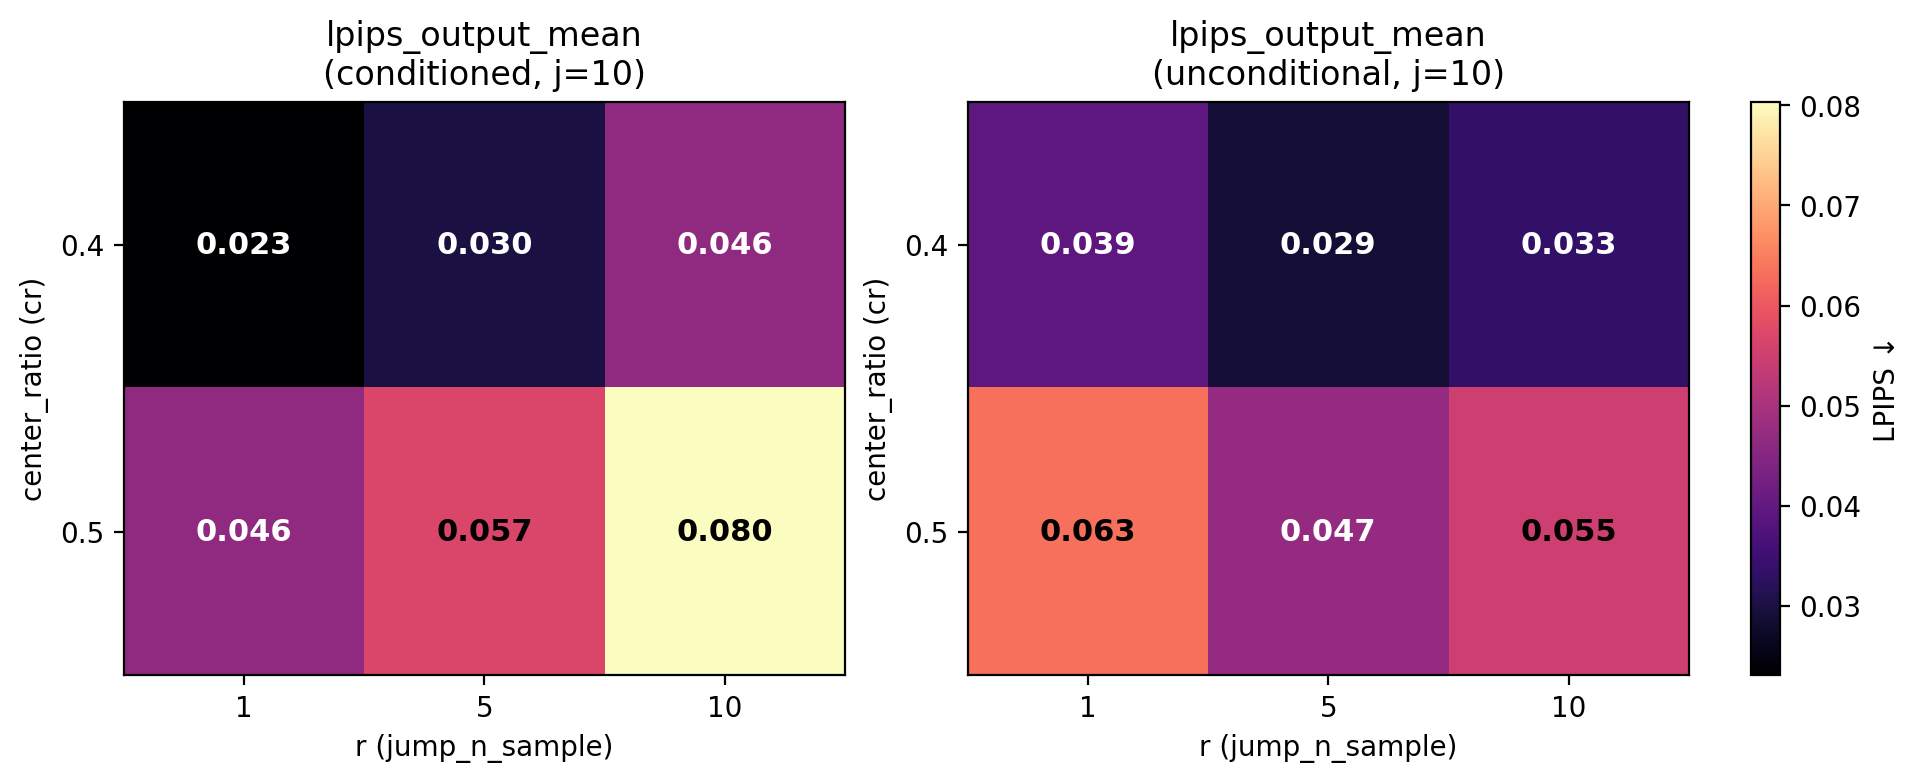
\includegraphics[width=0.98\linewidth]{figures/heatmap_lpips_output_mean_cr040_050_cond_vs_uncond_j10.png}
  \caption{Mean LPIPS (lower is better) over center-mask inpainting as a function of resampling count $r$ ($j{=}10$).
  Left: our conditioned DDPM. Right: our unconditional DDPM.
  Trends oppose: conditioned quality degrades with $r$; our unconditional quality improves from $r{=}1$ to $r{=}5$.}
  \label{fig:lpips-heatmap}
\end{figure}

\subsection{Qualitative evidence on our models}
\label{sec:qualitative}
Figures~\ref{fig:cond-r} and~\ref{fig:uncond-r} illustrate the same interaction on our own trained models.
Our conditioned outputs at $r{=}1$ are typically coherent; increasing to $r{=}10$ introduces washed-out / over-harmonized fills and visible degradation on several identities (Figure~\ref{fig:cond-r}).
Our unconditional model at $r{=}1$ often shows blotchy skin and hard seams; raising $r$ improves boundary harmony and facial structure (Figure~\ref{fig:uncond-r}).

\subsection{External qualitative check (RePaint CelebA-HQ)}
\label{sec:external}
Figure~\ref{fig:external-repaint} provides an independent check: RePaint's original pretrained (unconditional) CelebA-HQ checkpoint shows no comparable degradation under the same resampling sweep---in fact quality improves with $r$---suggesting the harm we observe on large centers is tied to \emph{mask conditioning} rather than to our specific architecture or training setup.
This figure is \textbf{not} our unconditional $64{\times}64$ model (Figure~\ref{fig:uncond-r}).
It uses RePaint's publicly released pretrained checkpoint at $256{\times}256$, with a respaced $T{=}100$ schedule, $j{=}10$, $r\in\{1,5,10\}$, and $n{=}8$ samples on a fixed identity with a lower-face (surgical-mask-style) hole.
The run is qualitative only (no PSNR/LPIPS) and should not be read as another cell of Table~\ref{tab:resampling-delta}.

% [H] preserves source order: external remnant above Figure 2, then brush + Table 2.
% Larger height fills the previous bottom gap on this page.
\begin{figure}[H]
  \centering
  \vspace{-0.5em}
  \begin{minipage}[t]{0.48\textwidth}
    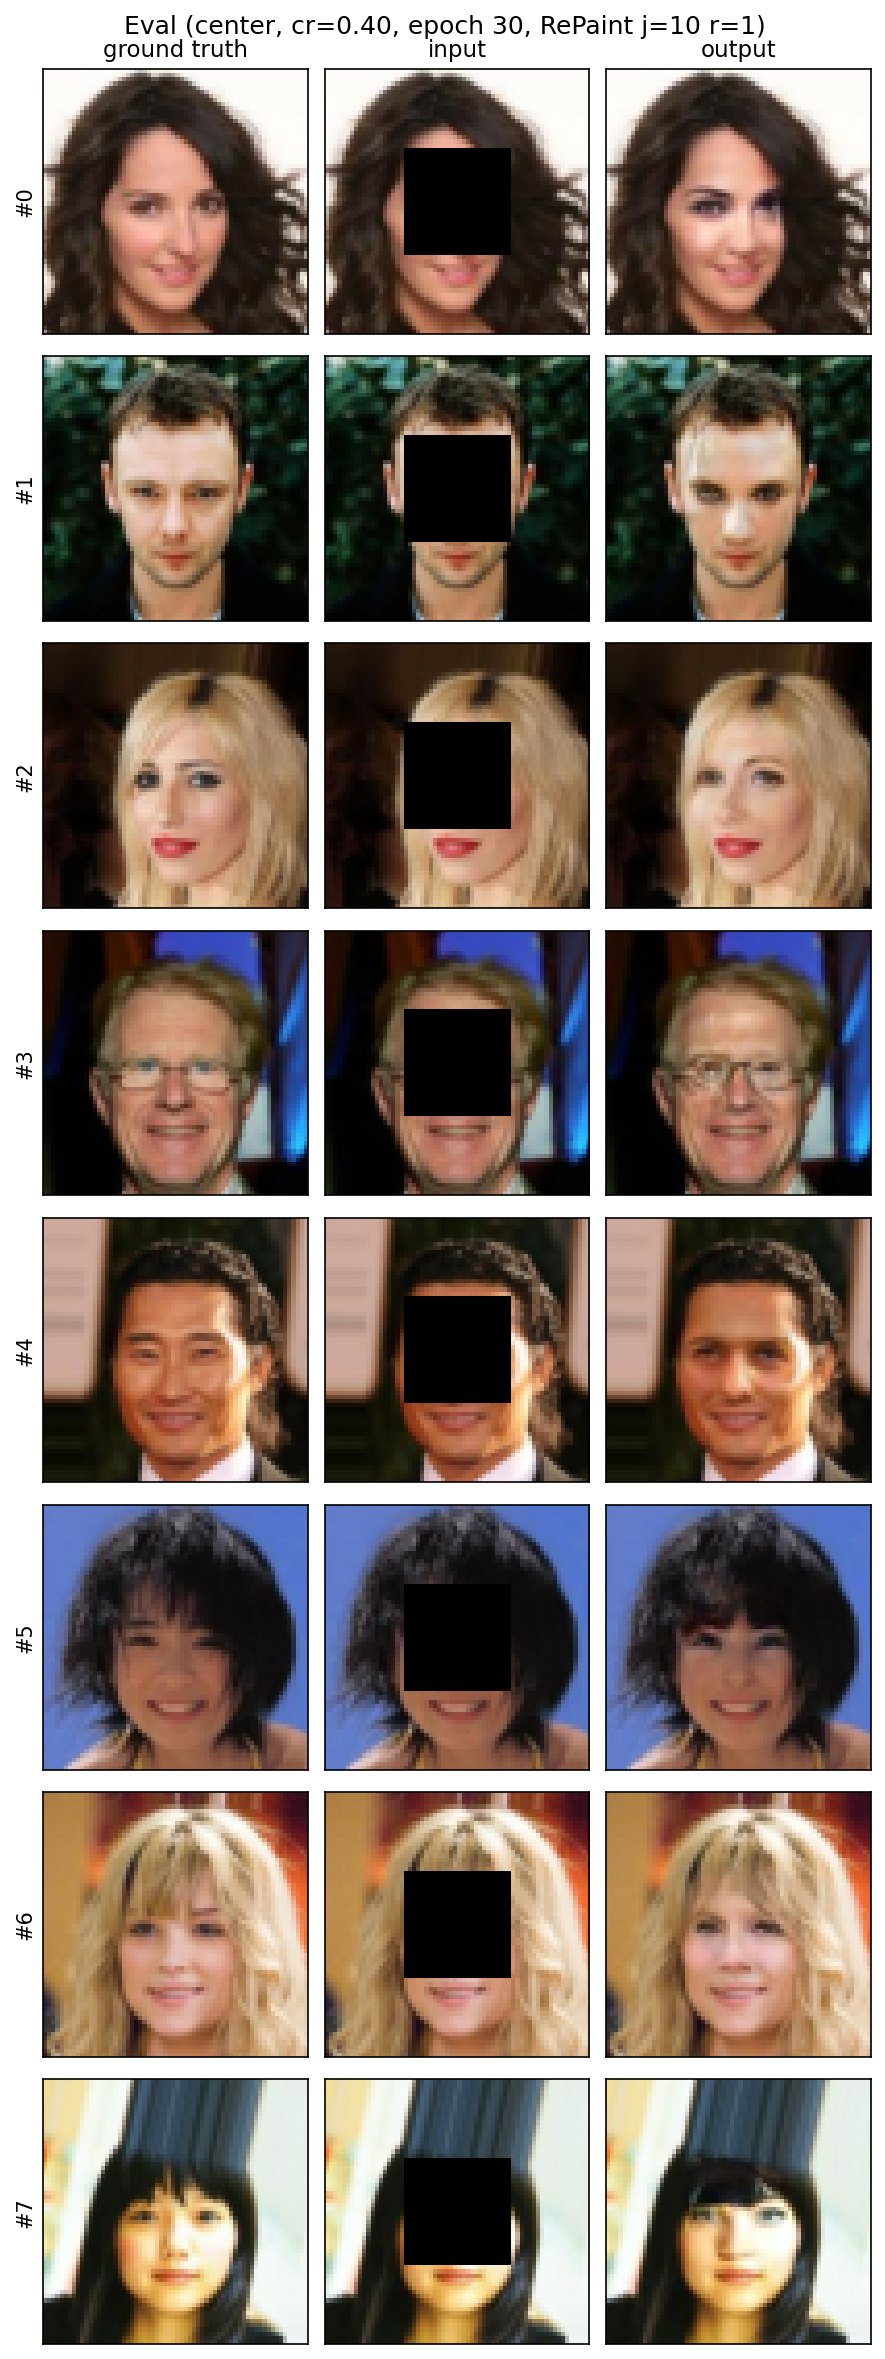
\includegraphics[width=\linewidth,height=0.41\textheight,keepaspectratio]{figures/eval_center_cr040_epoch_030_j10r1_grid.png}
    \vspace{-0.4em}
    \centerline{\small (a) Our conditioned, $r{=}1$}
  \end{minipage}
  \hfill
  \begin{minipage}[t]{0.48\textwidth}
    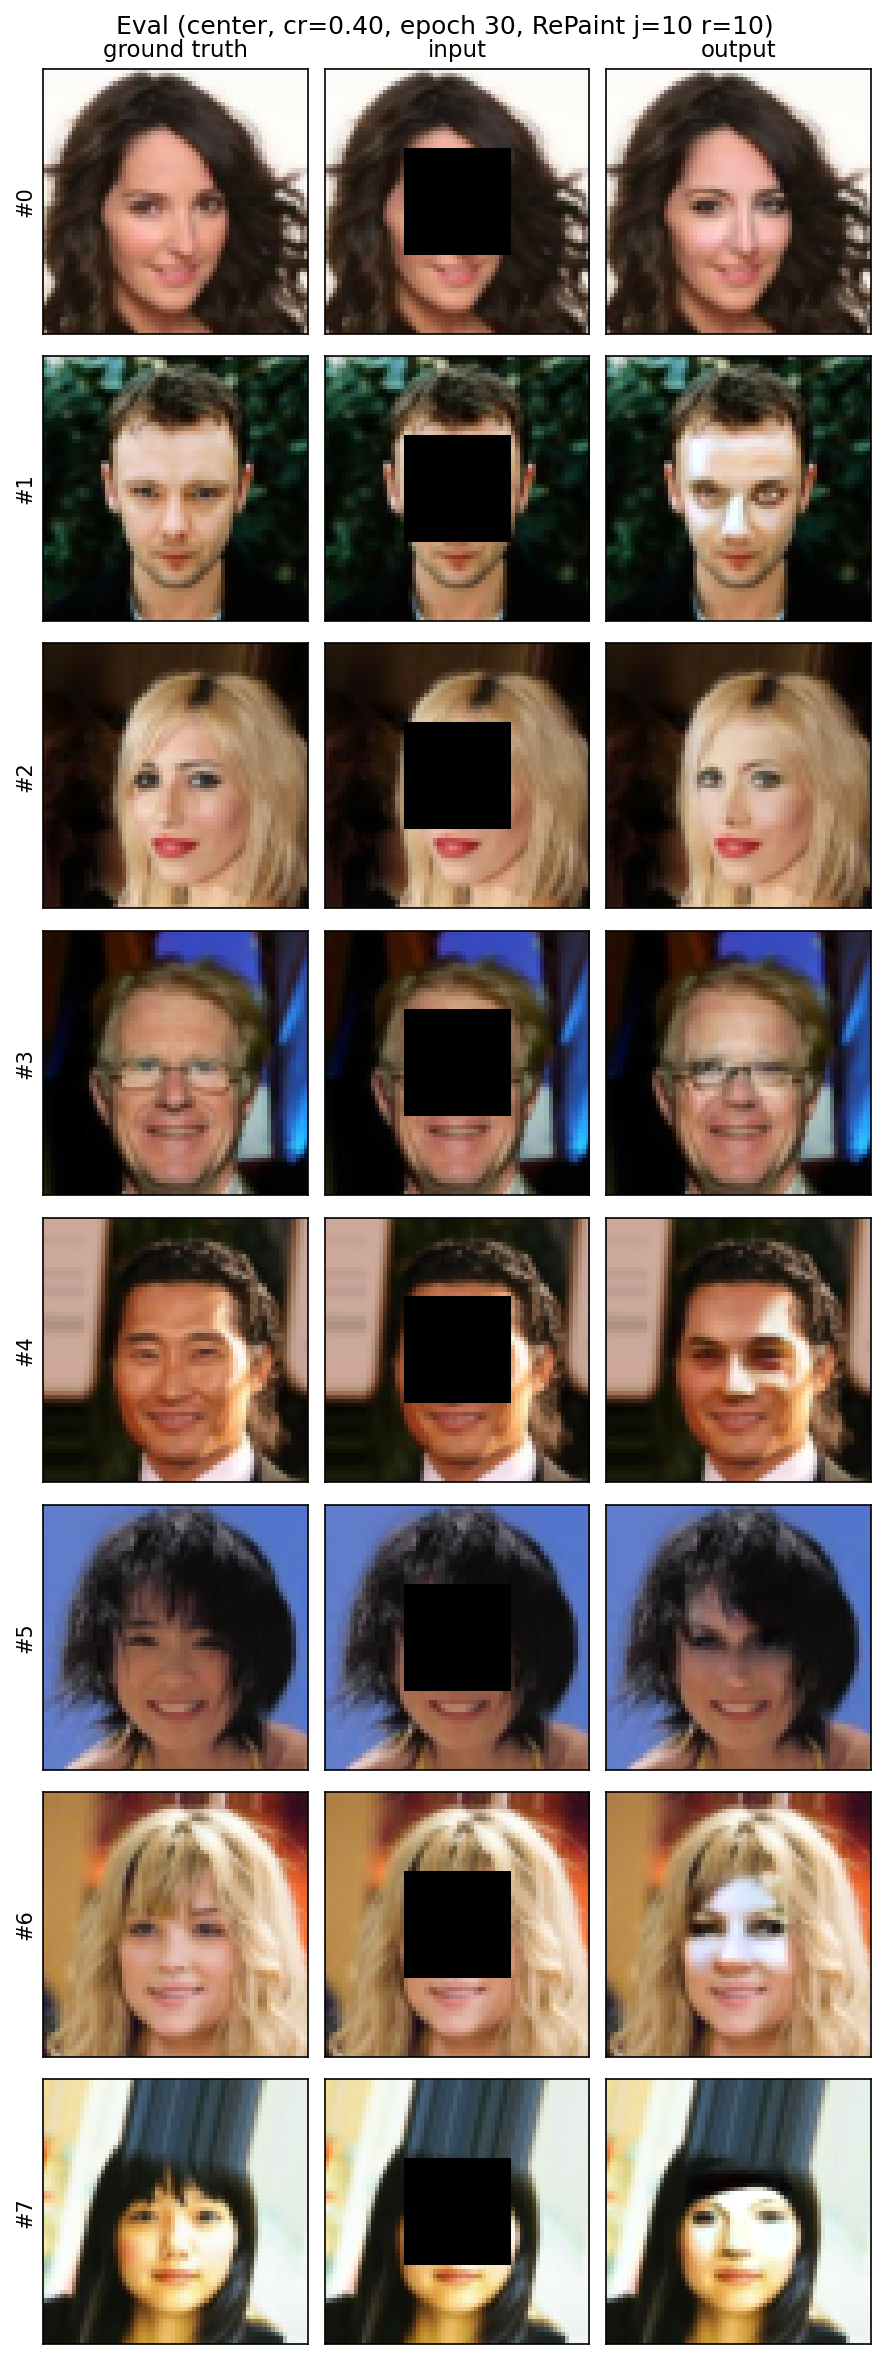
\includegraphics[width=\linewidth,height=0.41\textheight,keepaspectratio]{figures/eval_center_cr040_epoch_030_j10r10_grid.png}
    \vspace{-0.4em}
    \centerline{\small (b) Our conditioned, $r{=}10$}
  \end{minipage}
  \caption{Our conditioned CelebA model (epoch~$30$, $64{\times}64$), center $\mathrm{cr}{=}0.40$, $j{=}10$, full $T{=}1000$.
  Increasing $r$ from $1$ to $10$ tends to hurt fill quality.}
  \label{fig:cond-r}
\end{figure}

\subsection{Brush-mask control: the effect is contiguous-hole specific}
\label{sec:brush-null}
A natural confound is masked \emph{area}: perhaps any hole with $\mathrm{cr}{\approx}0.40$ coverage would show the same conditioned $r$-harm.
To test this, we evaluate the conditioned epoch-$30$ model on \textbf{brush} masks whose coverage is matched to a $\mathrm{cr}{=}0.40$ center hole, using the same paired protocol ($n{=}32$, $j{=}10$, $\Delta{=}\mathrm{metric}(r{=}10)-\mathrm{metric}(r{=}1)$, per-sample reseeding).
Table~\ref{tab:brush-null} reports a clean \textbf{null}.
Mean PSNR is essentially unchanged ($38.13\to38.43$\,dB):
$\Delta\mathrm{PSNR}{=}{+}0.30$\,dB with a 95\% CI that includes zero ($[{-}0.61,{+}1.20]$), $p{=}0.51$, and a negligible effect size (Cohen's $d{=}{+}0.12$).
$\Delta$LPIPS is likewise non-significant ($p{=}0.25$, $d{=}{+}0.21$).
Hole-PSNR differences match image-PSNR exactly under this protocol, as expected when only the masked region changes.
Increasing $r$ therefore neither reliably helps nor hurts under sparse, non-contiguous occlusion at matched coverage---while still costing ${\approx}10{\times}$ NFEs/$\,$wall-clock (Section~\ref{sec:cost}).
This rules out ``masked pixel count alone'' as the explanation for Table~\ref{tab:resampling-delta}:
the conditioned degradation under resampling is specific to \emph{large contiguous} holes, where RePaint's repeated re-harmonization has a coherent region to overwrite, not to brush strokes that leave dense local context.

\begin{table}[H]
  \centering
  \caption{Brush-mask control on the conditioned epoch-$30$ model ($n{=}32$, $j{=}10$).
  Coverage matched to center $\mathrm{cr}{=}0.40$.
  $\Delta{=}\mathrm{metric}(r{=}10)-\mathrm{metric}(r{=}1)$.
  Neither PSNR nor LPIPS changes significantly.}
  \label{tab:brush-null}
  \begin{tabular}{lcccc}
    \toprule
    Metric & $\Delta$ & 95\% CI & $p$ & Cohen's $d$ \\
    \midrule
    PSNR (dB) & $+0.30$ & $[-0.61,+1.20]$ & $0.51$ & $+0.12$ \\
    LPIPS & $+0.0006$ & $[-0.0005,+0.0017]$ & $0.25$ & $+0.21$ \\
    \bottomrule
  \end{tabular}
\end{table}

% No \clearpage here: prior \clearpage + oversized [H] produced a blank page.
\begin{figure}[H]
  \centering
  \begin{minipage}[t]{0.48\textwidth}
    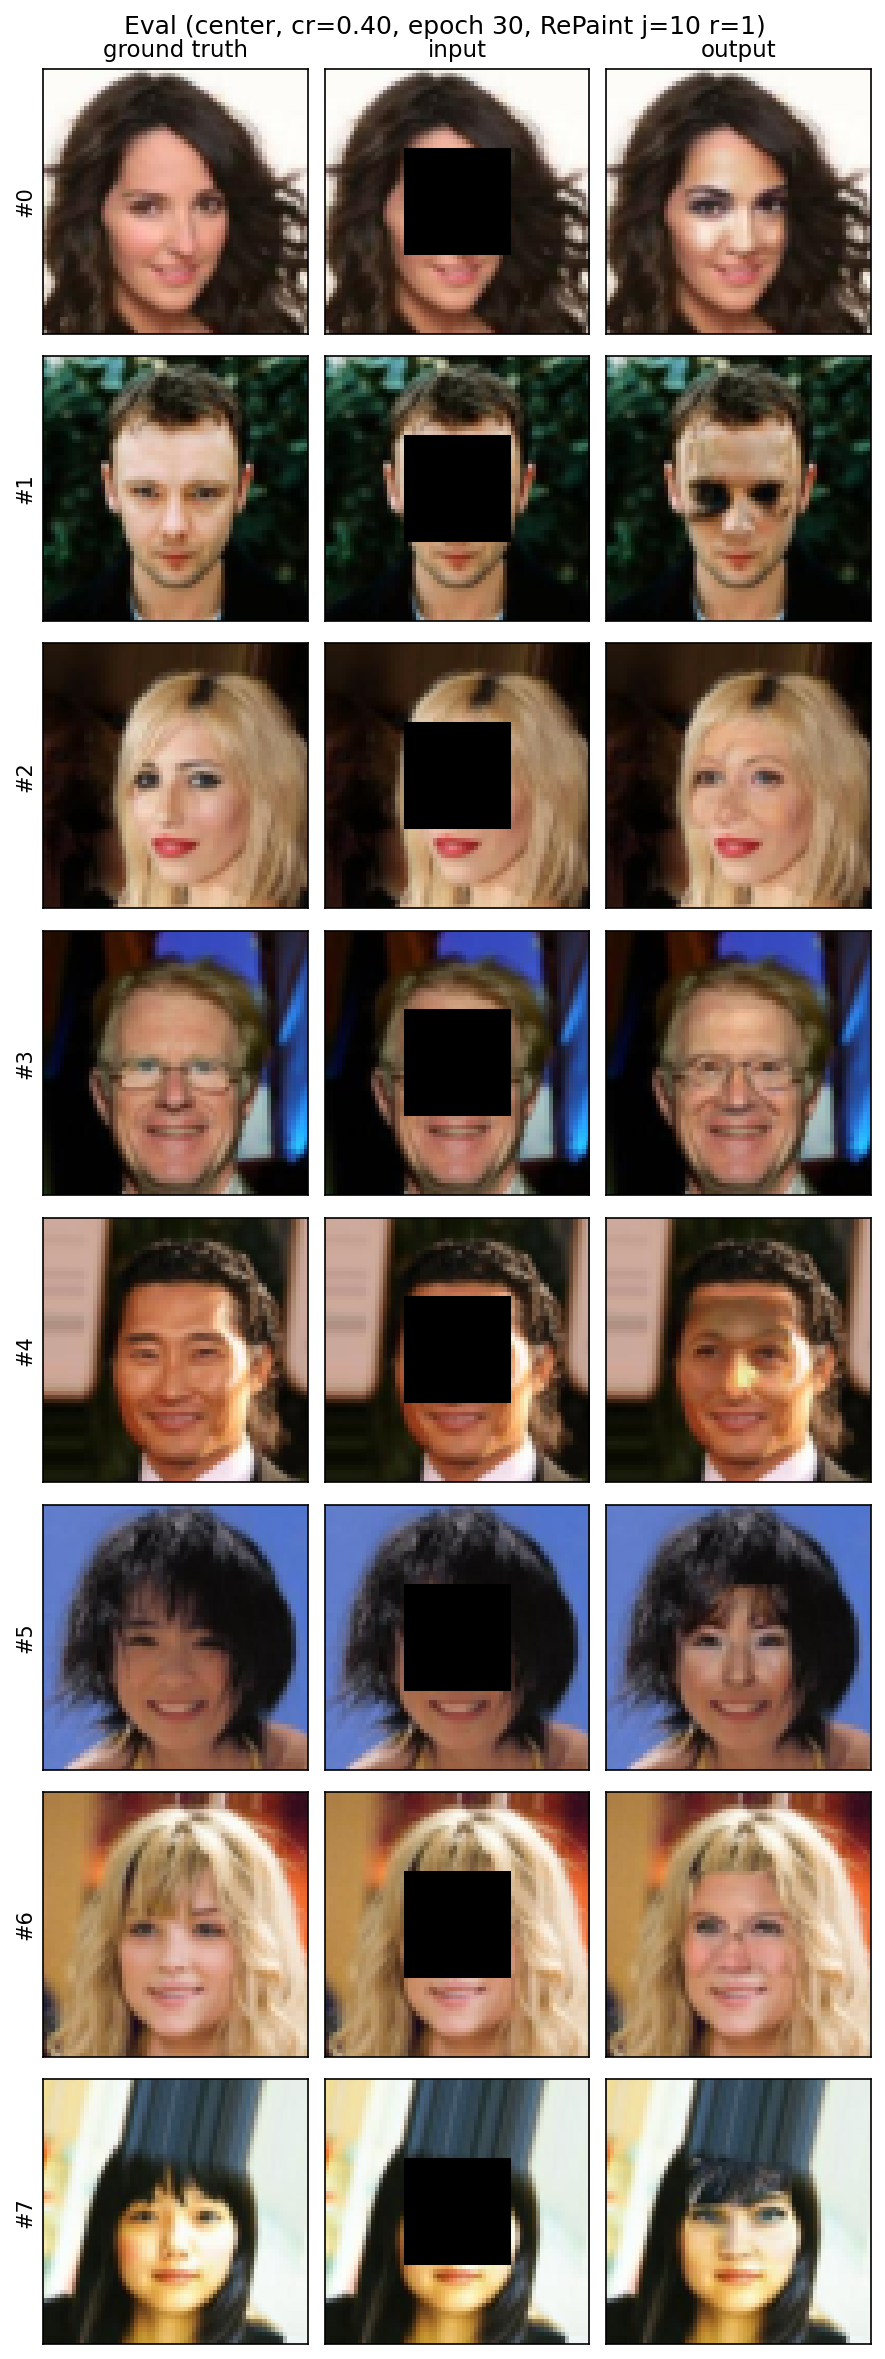
\includegraphics[width=\linewidth,height=0.40\textheight,keepaspectratio]{figures/eval_center_cr040_epoch_030_j10r1_uncond_grid.png}
    \vspace{-0.4em}
    \centerline{\small (a) Our unconditional, $r{=}1$}
  \end{minipage}
  \hfill
  \begin{minipage}[t]{0.48\textwidth}
    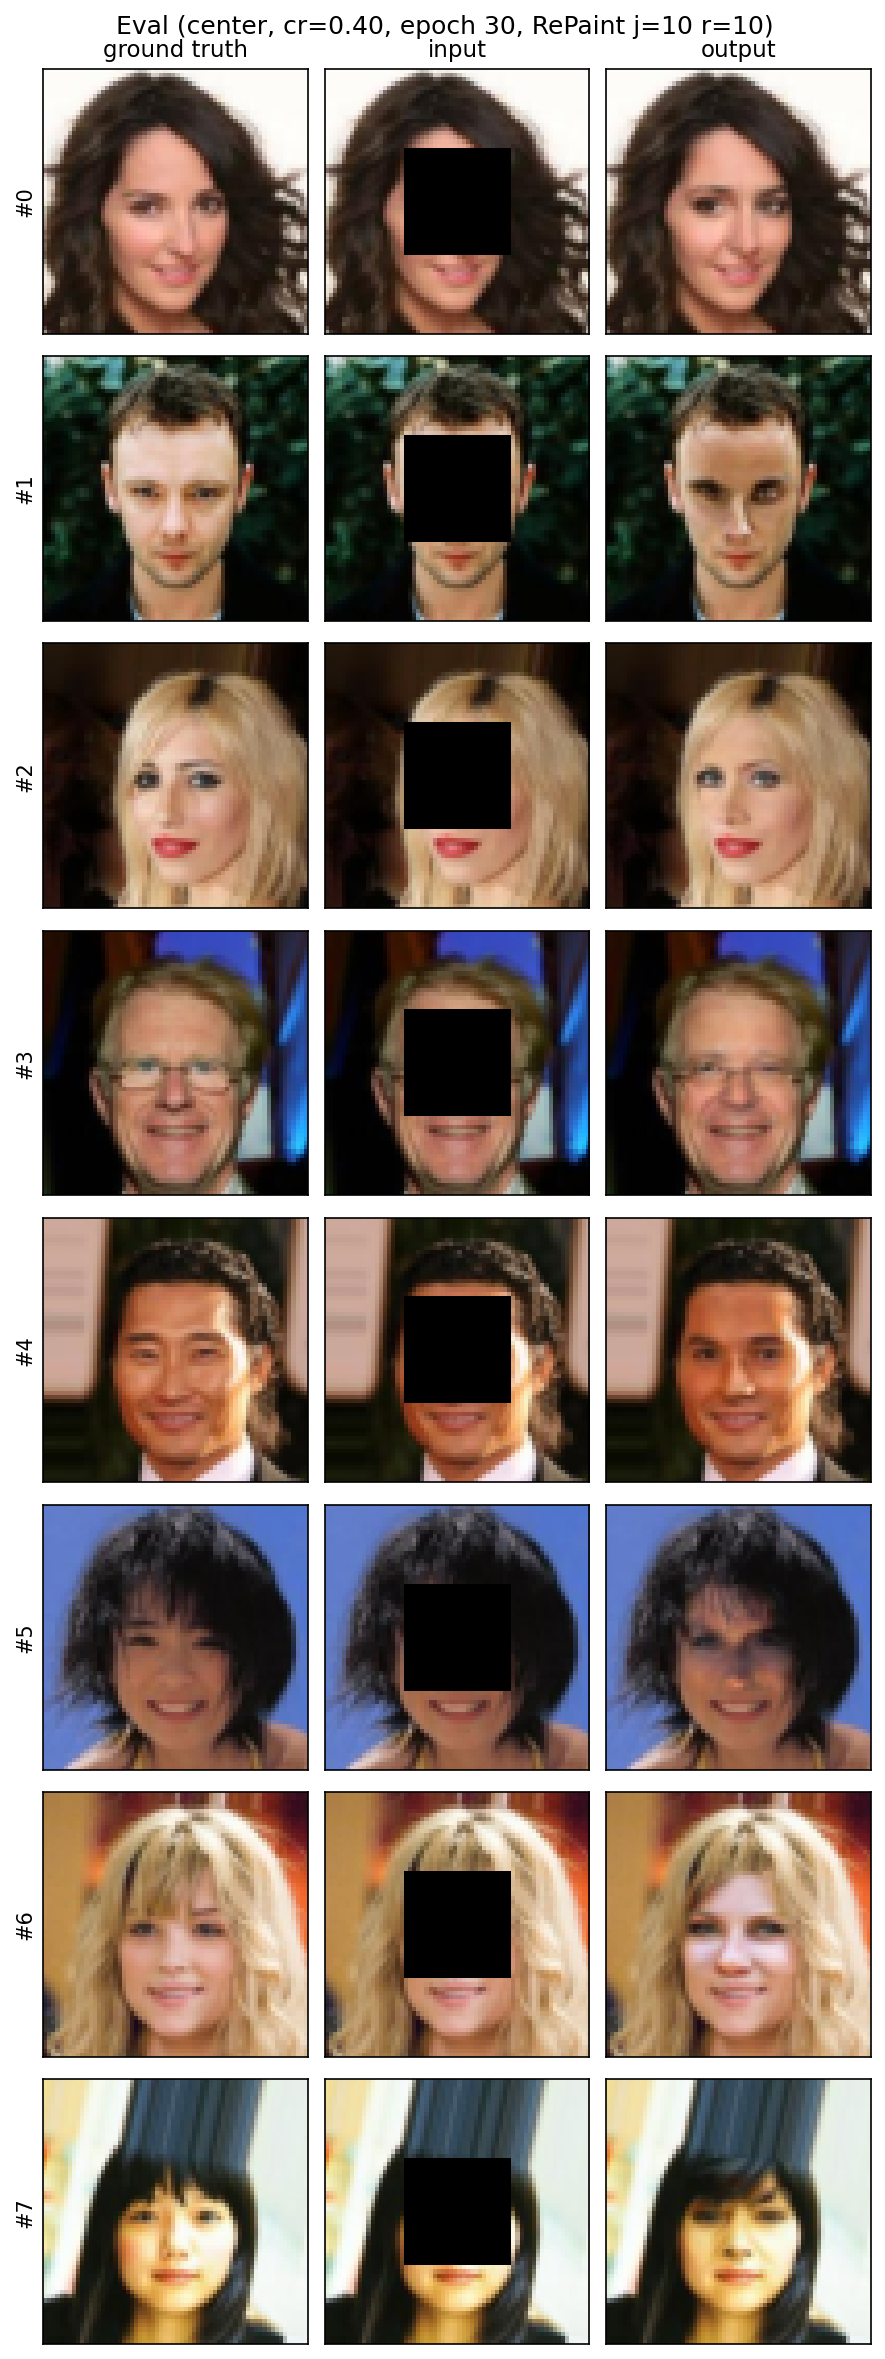
\includegraphics[width=\linewidth,height=0.40\textheight,keepaspectratio]{figures/eval_center_cr040_epoch_030_j10r10_uncond_grid.png}
    \vspace{-0.4em}
    \centerline{\small (b) Our unconditional, $r{=}10$}
  \end{minipage}
  \caption{Our unconditional CelebA model (epoch~$30$, $64{\times}64$), center $\mathrm{cr}{=}0.40$, $j{=}10$, full $T{=}1000$.
  Higher $r$ improves harmony relative to $r{=}1$ (Table~\ref{tab:resampling-delta} uses $r{=}5$ as the endpoint for our unconditional model).}
  \label{fig:uncond-r}

  \vspace{0.3em}

  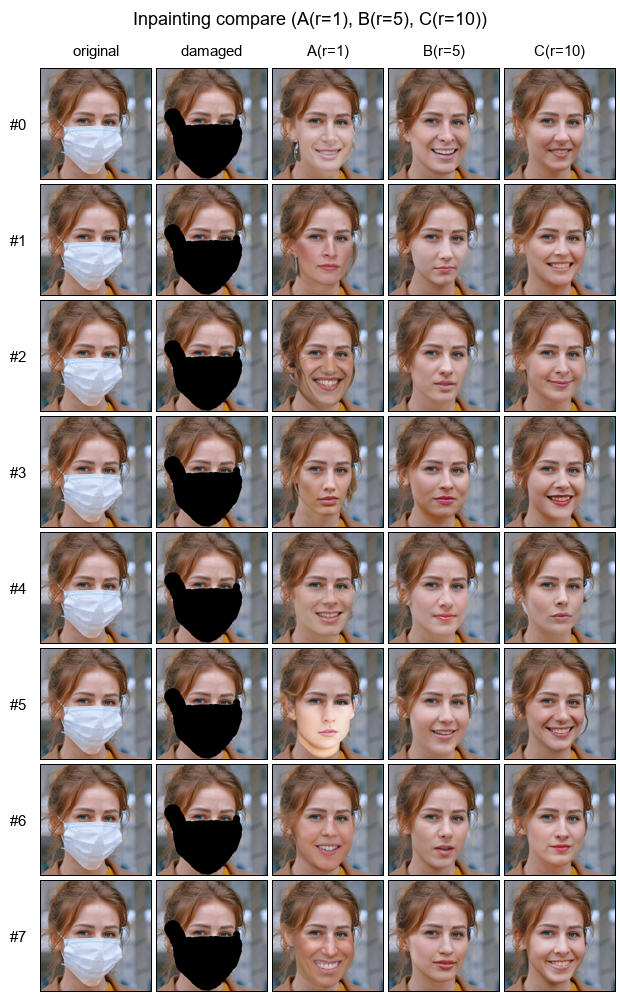
\includegraphics[width=0.98\textwidth,height=0.40\textheight,keepaspectratio]{figures/compare_ABC_grid.png}
  \caption{External qualitative check: RePaint's pretrained unconditional CelebA-HQ checkpoint ($256{\times}256$), \emph{not} our unconditional epoch-$30$ $64{\times}64$ model.
  Fixed identity, lower-face mask, respaced $T{=}100$, $j{=}10$, $n{=}8$.
  Columns: $r{=}1$, $r{=}5$, $r{=}10$.
  Higher $r$ improves seam consistency; unlike our conditioned model, there is no $r$-induced degradation.}
  \label{fig:external-repaint}
\end{figure}

\subsection{Compute cost of resampling}
\label{sec:cost}
Table~\ref{tab:nfe-cost} reports wall-clock and NFE cost as a function of $r$.

\begin{table}[H]
  \centering
  \caption{Inference cost vs.\ resampling count $r$ ($T{=}1000$, $j{=}10$). Ratios are relative to $r{=}1$.}
  \label{tab:nfe-cost}
  \begin{tabular}{rrrrr}
    \toprule
    $r$ & NFEs & NFE ratio & Wall-clock (s/img) & Time ratio \\
    \midrule
    $1$  & $1{,}000$ & $1.0{\times}$ & $14.1$ & $1.0{\times}$ \\
    $5$  & $4{,}960$ & $5.0{\times}$ & $70.8$ & $5.0{\times}$ \\
    $10$ & $9{,}910$ & $9.9{\times}$ & $149.7$ & $10.6{\times}$ \\
    \bottomrule
  \end{tabular}
\end{table}

Cost scales nearly linearly: $r{=}10$ requires ${\approx}9.9{\times}$ U-Net calls and ${\approx}10.6{\times}$ wall-clock time relative to $r{=}1$.
Combined with Table~\ref{tab:resampling-delta}, this yields a sharp practical conclusion for conditioned models: increasing $r$ can simultaneously \emph{worsen} quality and multiply inference cost by an order of magnitude.
For our unconditional model, moderate resampling ($r{=}5$) remains the operating point that improves quality, at about $5{\times}$ the cost of $r{=}1$.

\subsection{Takeaway}
\label{sec:takeaway}
RePaint resampling is not a universally beneficial hyperparameter.
Under matched seeds and identical images, its sign flips with the training regime: it helps the unconditional prior (as in the original RePaint setting) but hurts a mask-conditioned DDPM that already observes $(\tilde{x}_0,m)$ during reverse sampling.
The brush-mask null (Section~\ref{sec:brush-null}) further shows that the conditioned harm is tied to contiguous hole geometry, not coverage alone.
Reporting a single default $(j,r)$ across both regimes therefore conflates two different operating regimes---and, for conditioned models on large centers, can purchase worse images at substantially higher compute.
